\documentclass[12pt]{article}
\usepackage{Sweave}
\usepackage{amsmath}
\usepackage{bm}
\usepackage[authoryear,round]{natbib}
\bibliographystyle{plainnat}
 \DefineVerbatimEnvironment{Sinput}{Verbatim}
 {formatcom={\vspace{-2.5ex}},fontshape=sl,
   fontfamily=courier,fontseries=b, fontsize=\scriptsize}
 \DefineVerbatimEnvironment{Soutput}{Verbatim}
 {formatcom={\vspace{-2.5ex}},fontfamily=courier,fontseries=b,%
   fontsize=\scriptsize}
 
%\VignetteIndexEntry{Introduction to BioCro}
%\VignettePackage{BioCro}
  
\title{Simulation and Parameter Estimation for Biomass Crops}
\author{Fernando E. Miguez\\Energy Biosciences Institute\\
  University of Illinois}
\begin{document}


\setkeys{Gin}{width=\textwidth}
\newcommand{\code}[1]{\texttt{\small{#1}}}
\newcommand{\package}[1]{\textsf{\small{#1}}}
\maketitle
\begin{abstract}
Simulation and parameter estimation of photosynthesis and crop growth.
\end{abstract}


\section{Introduction}

This was started with the idea of being able to estimate parameters of
models used to simulate different aspect of the growth of a generic
crop. The model itself is largely based on WIMOVAC although it has
been completely re-written. Thus, this package does not only simulate
growth of crops but is also provides optimization routines for
parameter estimation. In addition, it uses the \package{lattice} for
building custom graphics.

A simple example follows

\begin{Schunk}
\begin{Sinput}
> data(weather05)
> res <- BioGro(weather05)
> res
\end{Sinput}
\begin{Soutput}
   DayofYear          Hour            Leaf               Stem          
 Min.   :123.0   Min.   : 0.00   Min.   :0.002548   Min.   : 0.009072  
 1st Qu.:168.0   1st Qu.: 6.00   1st Qu.:2.214368   1st Qu.: 7.262706  
 Median :212.0   Median :12.00   Median :3.302253   Median :18.070772  
 Mean   :212.5   Mean   :11.50   Mean   :2.779168   Mean   :15.890269  
 3rd Qu.:257.0   3rd Qu.:18.00   3rd Qu.:3.499368   3rd Qu.:24.091476  
 Max.   :301.0   Max.   :23.00   Max.   :3.533489   Max.   :27.658747  
      Root            Rhizome           Grain        LAI         
 Min.   :0.00868   Min.   : 2.617   Min.   :0   Min.   :0.00119  
 1st Qu.:2.74663   1st Qu.: 3.709   1st Qu.:0   1st Qu.:3.76397  
 Median :2.88269   Median : 5.941   Median :0   Median :5.61348  
 Mean   :2.59207   Mean   : 6.144   Mean   :0   Mean   :4.72410  
 3rd Qu.:2.97032   3rd Qu.: 8.257   3rd Qu.:0   3rd Qu.:5.94893  
 Max.   :3.03767   Max.   :10.614   Max.   :0   Max.   :6.00693  
    ThermalT        
 Min.   :   0.2090  
 1st Qu.: 865.7519  
 Median :1961.2109  
 Mean   :1940.2779  
 3rd Qu.:3038.9036  
 Max.   :3746.7109  
\end{Soutput}
\end{Schunk}

First, an example data set was loaded using the \code{data}
function. Then an object called \code{res} was created which stores
the result of running the function \code{BioGro} with the weather data
as input. The printing method displays only some of the relevant
information of the simulation. The function \code{BioGro} has many
options and the documentation is a good place to start to inquire
further (try \code{?BioGro}).

The plotting method provides a convenient way of displaying the results.

\begin{Schunk}
\begin{Sinput}
> plot(res)
\end{Sinput}
\end{Schunk}
\begin{figure}[htbp!]
  \centering
  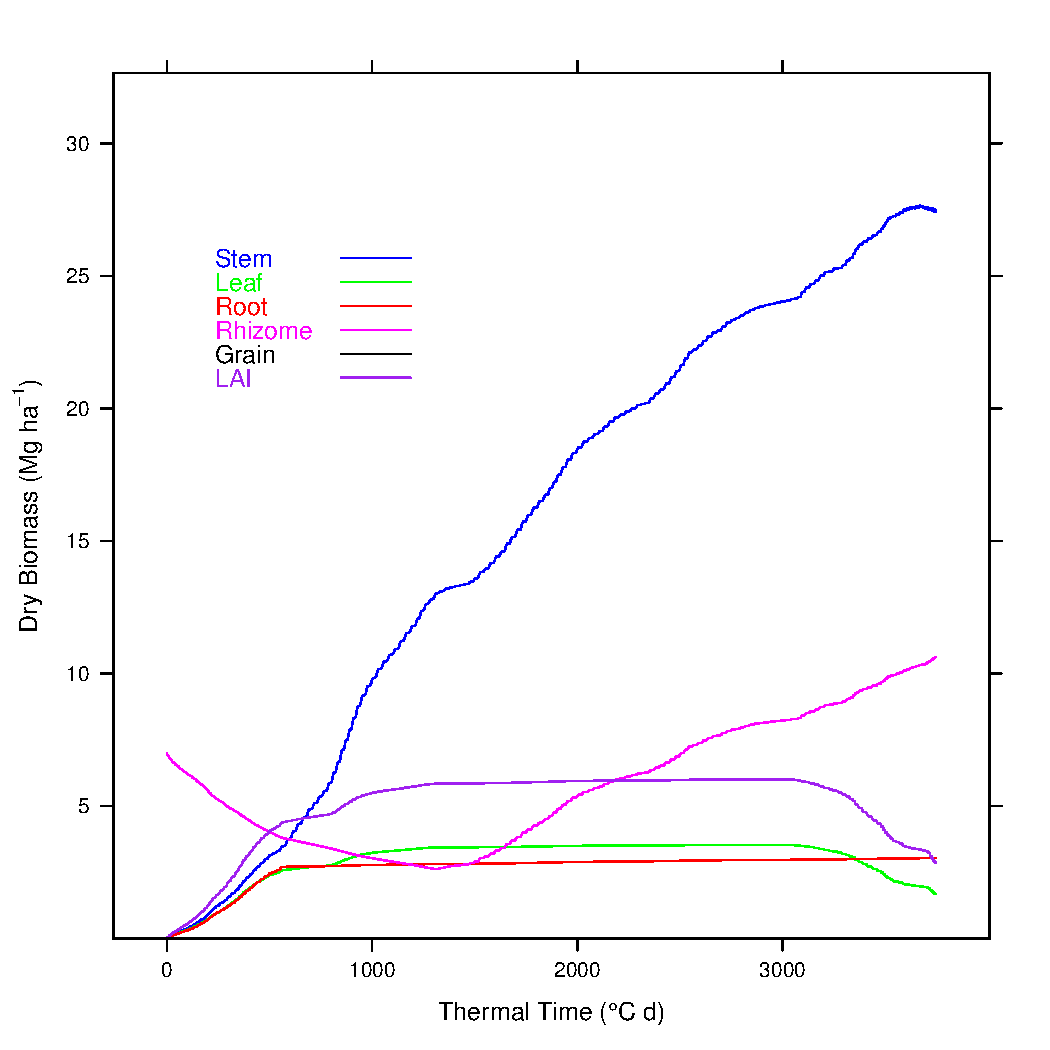
\includegraphics[scale=0.8]{./figs/BioCro-plotBioGro.pdf}
  \caption{Dry biomass accumulation and Leaf Area Index for a generic biomass crop against thermal time.}
  \label{fig:plotBioGro}
\end{figure}

\section{Parameter Estimation}

Often the carbon allocation needs to be modeled from samples of
biomass including stem, leaf, rhizome and root. To evaluate the
ability of the model to recover the `true' coefficients some data were
simulated.

\begin{Schunk}
\begin{Sinput}
> data(weather05)
> pheno.ll <- phenoParms(kLeaf1 = 0.48, kStem1 = 0.47, kRoot1 = 0.05, 
+     kRhizome1 = -1e-04, kLeaf2 = 0.14, kStem2 = 0.65, kRoot2 = 0.21, 
+     kRhizome2 = -1e-04, kLeaf3 = 0.01, kStem3 = 0.56, kRoot3 = 0.13, 
+     kRhizome3 = 0.3, kLeaf4 = 0.01, kStem4 = 0.56, kRoot4 = 0.13, 
+     kRhizome4 = 0.3, kLeaf5 = 0.01, kStem5 = 0.56, kRoot5 = 0.13, 
+     kRhizome5 = 0.3, kLeaf6 = 0.01, kStem6 = 0.56, kRoot6 = 0.13, 
+     kRhizome6 = 0.3)
> system.time(ans <- BioGro(weather05, phenoControl = pheno.ll))
> dbp.ll <- phenoParms()
> tts6 <- c(1, 500, 1300, 2000, 2600, 3200, 3700)
> indx <- BioCro:::indfun(tts6, ans$ThermalT)
> ans.dat <- as.data.frame(unclass(ans)[1:11])
> sel.rows <- indx
> simDat <- ans.dat[sel.rows, c("ThermalT", "Stem", "Leaf", "Root", 
+     "Rhizome", "Grain", "LAI")]
> ans0 <- BioGro(weather05)
> rss0 <- RssBioGro(simDat, ans0)
> idb <- valid_dbp(idbp(simDat))
> op1 <- OpBioGro(phen = 0, WetDat = weather05, data = simDat, 
+     iCoef = idb, op.method = "optim")
> dbp.ll[7:31] <- op1$coefs
> ans1 <- BioGro(weather05, phenoControl = dbp.ll)
> (rss1 <- RssBioGro(simDat, ans1))
> (dist1 <- dist(rbind(op1$coefs, as.vector(unlist(pheno.ll)[7:31]))))
> (nconv1 <- length(op1$opar$convergence[op1$opar$convergence == 
+     0]))
\end{Sinput}
\end{Schunk}


% \section{Simulating Photosynthesis}
% \label{sec:simphoto}

% The package has only two functions at the time. The first one of interest is
% \texttt{c3photo}. Let us see what the arguments for this function are

% <<<argC3photo>>=
% args(c3photo)
% @ 

% \texttt{Qp} is the quantum flux, \texttt{Tl} is the temperature of the
% leaf, \texttt{RH} is the relative humidity, \texttt{vcmax} is the
% maximum rate of carboxylation, \texttt{jmax} is the maximum rate of
% electron transport, \texttt{Rd} is the dark respiration, \texttt{Catm}
% is the atmospheric $CO_2$ concentration, \texttt{O2} is the
% atmospheric oxygen concentration, \texttt{b0} is the intercept of the
% Ball-Berry model, \texttt{b1} is the slope of the Ball-Berry model for
% stomatal conductance and \texttt{theta} is the curvature parameter for
% the light response. For more information see the function
% documentation (i.e. ?c3photo).

% <<C3photo,fig=TRUE,include=FALSE,echo=FALSE>>=
% Qps <- seq(0,2000,10)
% Tls <- seq(0,50,5)
% rhs <- c(0.7)
% dat1 <- data.frame(expand.grid(Qp=Qps,Tl=Tls,RH=rhs))
% res1 <- c3photo(dat1$Qp,dat1$Tl,dat1$RH) 
% res2 <- c3photo(dat1$Qp,dat1$Tl,dat1$RH,vcmax=120)

% plot1 <- xyplot(res1$Assim + res2$Assim ~ Qp | factor(Tl) , data = dat1,
%                type="l",col=c("blue","green"),lwd=2,
%                ylab=expression(paste("Assimilation (",
%                    mu,mol," ",m^-2," ",s^-1,")")),
%                xlab=expression(paste("Quantum flux (",
%                    mu,mol," ",m^-2," ",s^-1,")")),
%                key=list(text=list(c("Vcmax 100","Vcmax 120")),
%                  lines=TRUE,col=c("blue","green"),lwd=2))
% print(plot1)
% @
% \begin{figure}[htbp!]
%   \centering
%   \includegraphics{Intro-C3photo}
%   \caption{Assimilation response to light levels for different
%     temperatures (in Celsius).  Each panel is a different level of
%     temperature. The two lines within a panel show different values
%     for $Vcmax$.}
%   \label{fig:C3photo}
% \end{figure}

% \section{Optimizing Parameters for a single A/Ci curve}

% The other function of interest is \texttt{Opc3photo}. 

% <<Opc3photo>>=
% args(Opc3photo)
% @ 

% The \texttt{data} argument should be the observed assimilation
% data. One example is the built-in dataset \texttt{simA100}.

% <<simA100>>=
% data(simA100)
% head(simA100)
% @ 

% The dataset contains more than is needed to run \texttt{Opc3photo}. We
% know that this dataset was simulated and that the `true' values for
% $Vcmax$, $Jmax$, and $Rd$ are 90.8, 206, and 2.31 respectively. Can we
% recover them from the data alone?

% <<Opc30, eval=FALSE>>=
% Opc3photo(simA100[,1:5],Catm=simA100[,9], curve.kind="Ci", op.level=2)
% @ 
% <<Opc30,echo=FALSE>>=
% tmp <- try(Opc3photo(simA100[,1:5],Catm=simA100[,9], curve.kind="Ci", op.level=2),silent=TRUE)
% @ 
% <<echo=FALSE>>=
% if(class(tmp) == "try-error"){
%   cat(strwrap(tmp), sep="\n")
%   }else{
%     tmp
%     }
% @ 



% This is fabricated data and the function works even if the variance
% seems to be close zero. We can try a slower, less accurate method first to
% get starting values as well. And suppress the computation of the
% hessian.


% <<Opc3photo3>>=
% op100 <- Opc3photo(simA100[,1:5],Catm=simA100[,9], 
%                    method="SANN", hessian=FALSE,
%                    curve.kind="Ci", op.level = 2)
% @ 

% now we can use this values as starting values. If we do not specify
% the optimization method it will use the default used by the
% \texttt{optim} function which is ``Nelder-Mead'' (see \texttt{?optim}).


% <<Opc3photo4>>=
% op100 <- Opc3photo(simA100[,1:5],Catm = simA100[,9], 
%                    ivcmax = op100$bestVmax,
%                    ijmax = op100$bestJmax,
%                    iRd = op100$bestRd,
%                    curve.kind="Ci", op.level=2)
% op100
% @ 

% The small confidence intervals are a result of using fabricated data.
% We can examine the quality of the fit by plotting the residuals. The
% option \texttt{resid} is used to plot `raw' residuals as opposed to
% standardized.

% <<op100resid, eval=FALSE>>=
% plot(op100, resid="raw")
% @ 
% <<echo=FALSE, print=FALSE, term=FALSE>>=
% pdf("./figs/Intro-op100resid.pdf")
% plot(op100, resid="raw")
% dev.off()
% @
% \begin{figure}[htbp!]
%   \centering
%   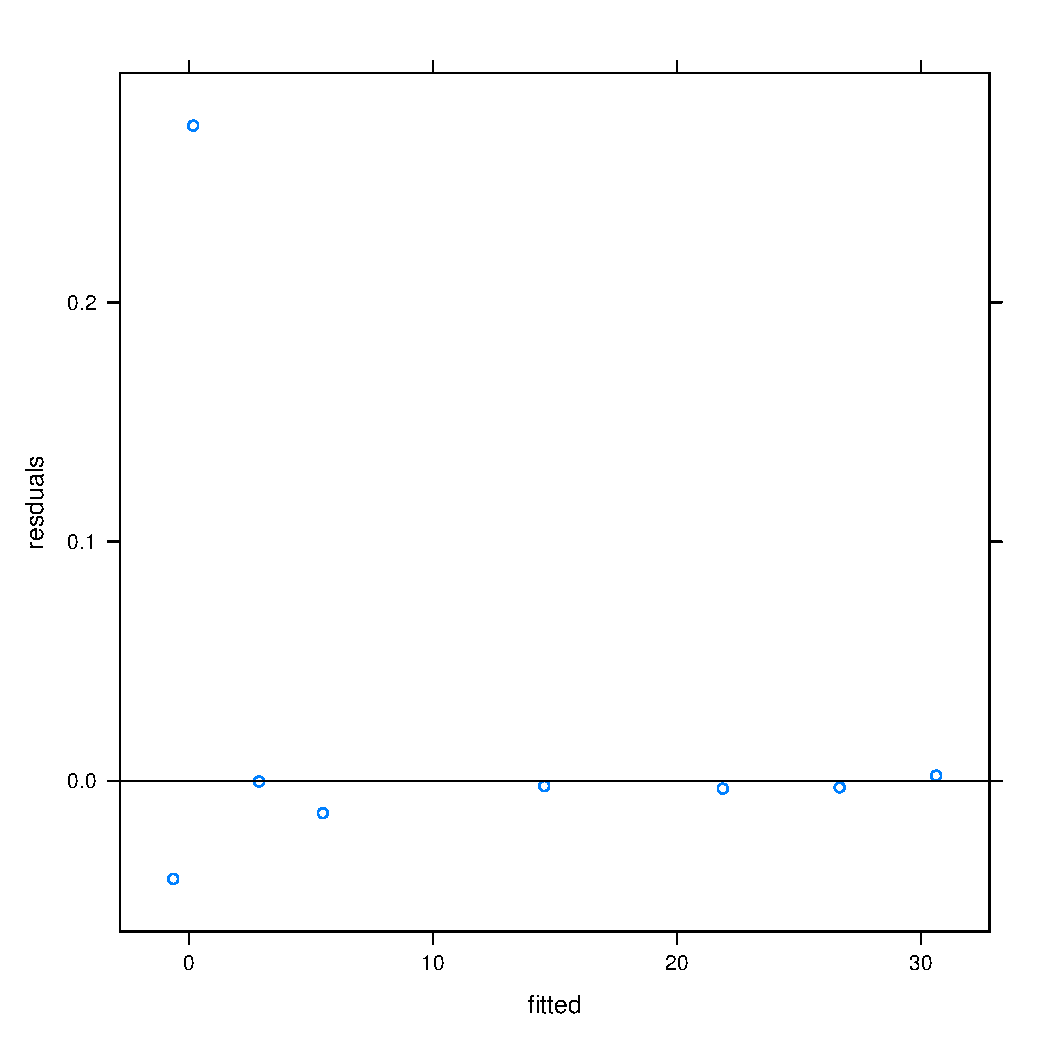
\includegraphics[scale=0.8]{./figs/Intro-op100resid}
%   \caption{Raw residuals for op100}
%   \label{fig:op100resid}
% \end{figure}

% The residuals show one outlier, but the deviations are
% small. The option \texttt{plot.kind} is used to plot the observed
% vs. fitted.

% <<op100, eval=FALSE>>=
% plot(op100, plot.kind="OvsF")
% plot(op100, plot.kind="OandF", type='o')
% @
% <<op100OvsF, echo=FALSE, print=FALSE, term=FALSE>>=
% pdf("./figs/Intro-op100-OvsF.pdf")
% plot(op100, plot.kind="OvsF")
% dev.off()
% pdf("./figs/Intro-op100-OandF.pdf")
% plot(op100, plot.kind="OandF", type='o')
% dev.off()
% @
% \begin{figure}[htbp!]
%   \centering
%   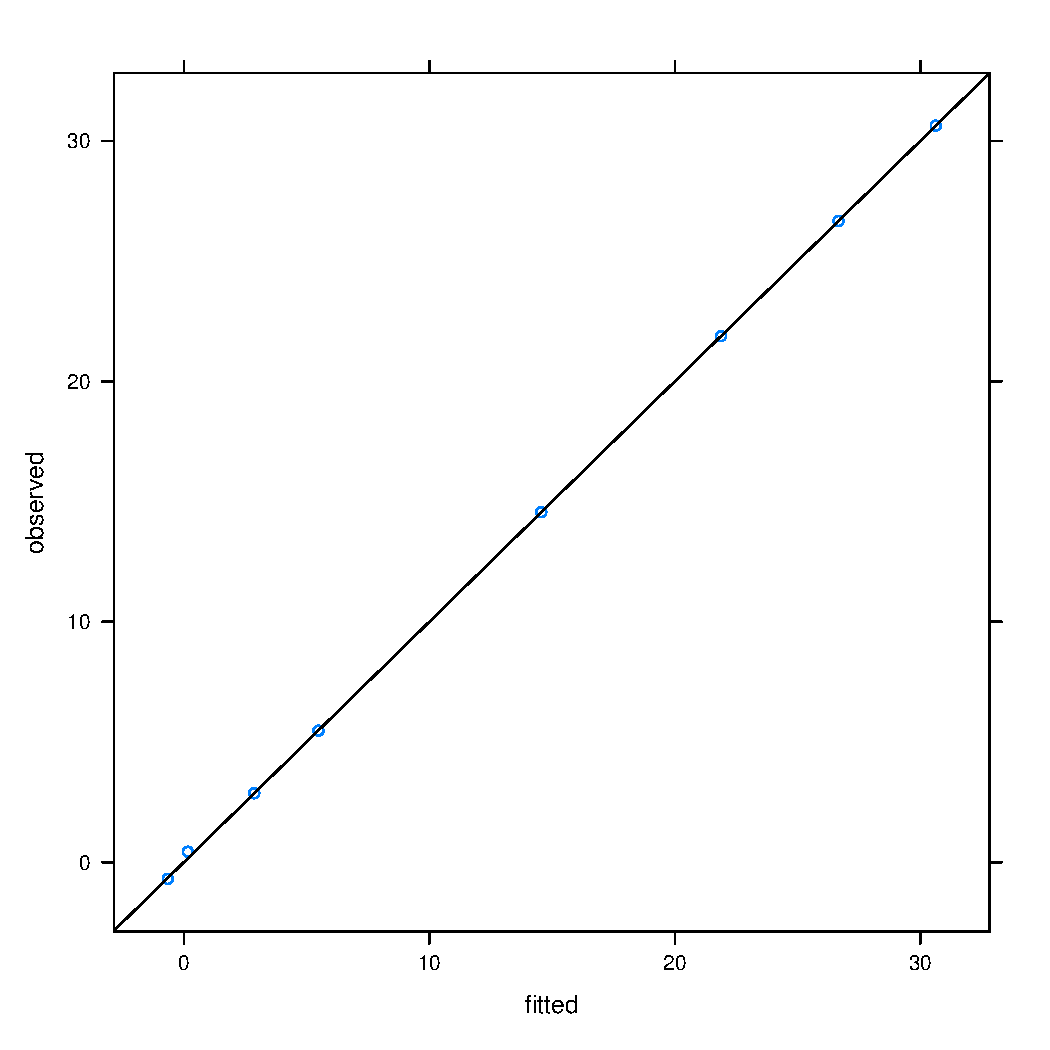
\includegraphics[scale=0.8]{./figs/Intro-op100-OvsF}  
%   \caption{Observed vs. fitted for the optimization on the simulated data.}
%   \label{fig:ovsf}
% \end{figure}

% \begin{figure}[htbp!]
%   \centering
%   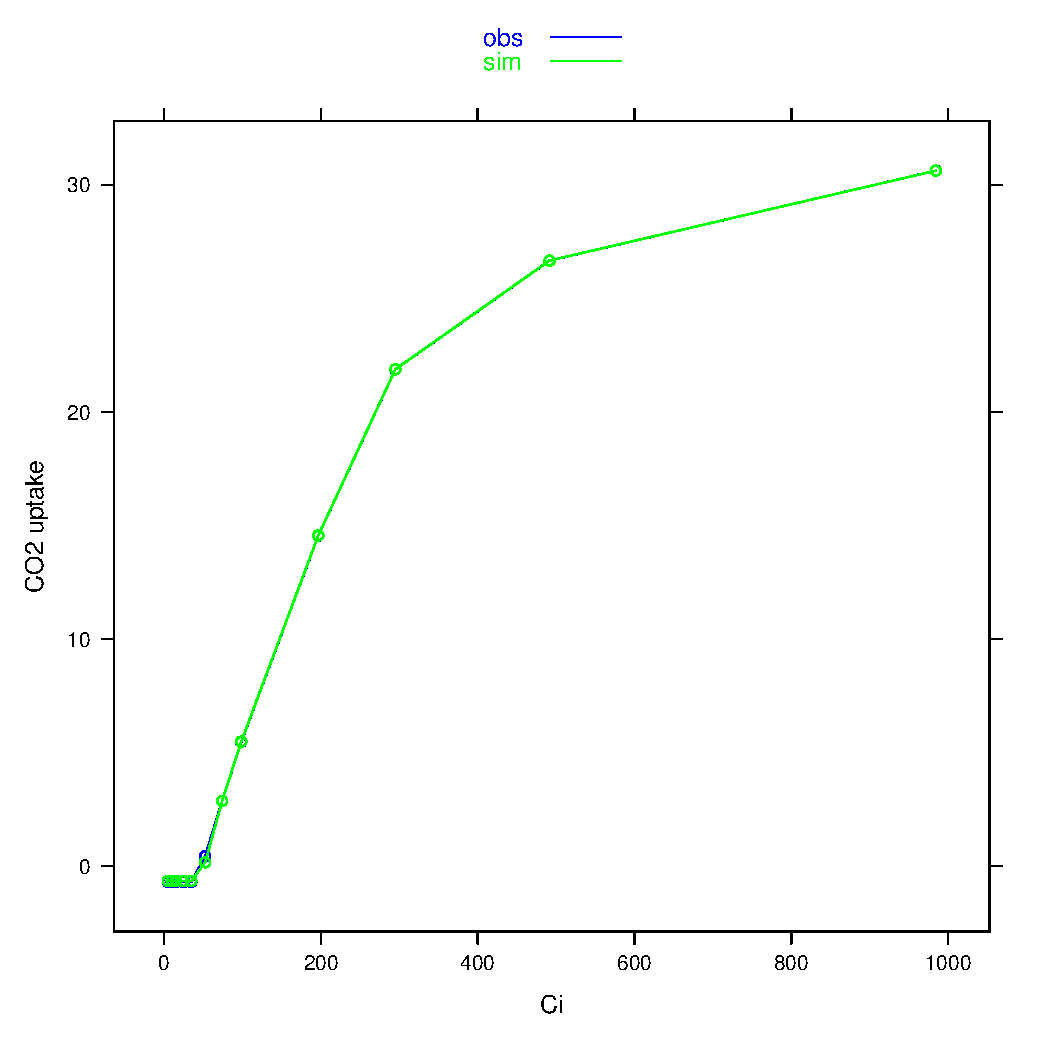
\includegraphics[scale=0.8]{./figs/Intro-op100-OandF}  
%   \caption{Observed and fitted for the optimization on the simulated data.}
%   \label{fig:oandf}
% \end{figure}


% This function can optimize photosynthesis considering assimilation and
% intercellular $CO_2$ both as outputs of the model, but this should be
% done only for `slow-measured' curves. For $A/C_i$ curves the values of
% atmospheric $CO_2$ should also be supplied. The fifth column with
% $C_i$ values is optional. This allows this optimization function to at
% least attempt to optimize any type of photosynthesis data including
% diurnals, temperature response functions and $A/Q$ curves as well. Not
% all data are suitable to estimate the three parameters shown here, so
% the optimization level could also be adjusted.

% \section{Optimizing Parameters for multiple $A/C_i$ curves}

% A wrapper function for \texttt{Opc3photo} called \texttt{mOpc3photo}
% can be used to optimize multiple $A/C_i$ curves which are considered
% multiple `runs'. An example dataset is included.
% \vspace*{0.5cm}

% <<simAssim>>=
% data(simAssim)
% head(simAssim)
% @ 

% These has more than we need, but it contains the `true' values used to
% generate the data so that we can later see if the optimization method
% can recover the `true' values of the parameters. For the optimization
% we need this format.
% \vspace*{0.5cm}

% <<simAssim2>>=
% simAssim2 <- cbind(simAssim[,1:6],Catm=simAssim[,10])
% head(simAssim2)
% parms <- simAssim[seq(1,3600,12),7:9]
% @ 

% The `true' parameters were stored in the parms object.  Now we can run
% the \texttt{mOpc3photo} function.
% \vspace*{0.5cm}

% <<mOpc3photo>>=
% op.all <- mOpc3photo(simAssim2, op.level=2)
% table(op.all[,4])
% @ 

% For the initial run we know that 1 runs did not converge, but this is
% expected as what we want with this first optimization is to get good
% starting values. If some of them did not converge we could replace
% missing values with the mean of each parameter, but this is not needed
% here.  \vspace*{0.5cm}

% <<apply>>=
% colm <- apply(op.all,2,mean,na.rm=TRUE)
% op.all[is.na(op.all[,1]),1] <- colm[1]
% op.all[is.na(op.all[,2]),2] <- colm[2]
% op.all[is.na(op.all[,3]),3] <- colm[3]
% @ 

% Now we can run it again.
% \vspace*{0.5cm}

% <<mOpc3photo2>>=
% op.all2 <- mOpc3photo(simAssim2, iVcmax=op.all[,1], iJmax=op.all[,2], iRd=op.all[,3], op.level=2)
% table(op.all2[,4])
% @ 

% Some of them might not converge, in this case all of them did. We can
% examine if each optimization was able to recover the true values.

% \vspace*{0.5cm}

% <<TvsEparms1,fig=TRUE>>=
% plot(parms[,1],op.all2[,1], ylim=c(70,110), xlim=c(70,110),
%      xlab="Obs (true)",ylab="Sim (est)",main="Vcmax")
% abline(0,1)
% @
% \begin{figure}[htbp!]
%   \centering
%   \includegraphics{Intro-TvsEparms1}
%   \caption{Agreement between true and estimated values for Vcmax}
%   \label{fig:tvseparms1}
% \end{figure}

% \vspace*{0.5cm}

% <<TvsEparms2,fig=TRUE>>=
% plot(parms[,2],op.all2[,2],xlab="Obs (true)",ylab="Sim (est)",main="Jmax")
% abline(0,1)
% @
% \begin{figure}[htbp!]
%   \centering
%   \includegraphics{Intro-TvsEparms2}
%   \caption{Agreement between true and estimated values for Jmax}
%   \label{fig:tvseparms2}
% \end{figure}

% \vspace*{0.5cm}

% <<TvsEparms3,fig=TRUE>>=
% plot(parms[,3],op.all2[,3],xlab="Obs (true)",ylab="Sim (est)",main="Rd")
% abline(0,1)
% @
% \begin{figure}[htbp!]
%   \centering
%   \includegraphics{Intro-TvsEparms3}
%   \caption{Agreement between true and estimated values for Rd}
%   \label{fig:tvseparms3}
% \end{figure}




\end{document}

